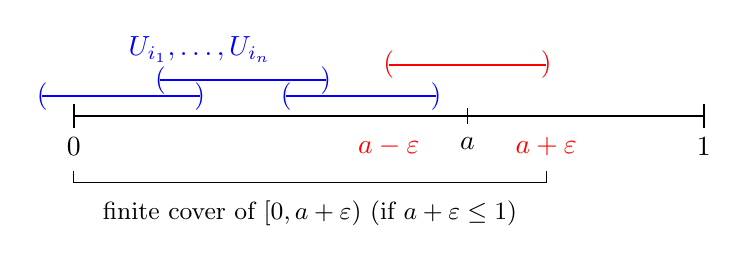
\begin{tikzpicture}
\draw[thick] (0,0) -- (8,0);
\draw[thick] (0,-0.15) -- (0,0.15); \draw[thick] (8,-0.15) -- (8,0.15);
\node[below] at (0,-0.15) {$0$};
\node[below] at (8,-0.15) {$1$};
\draw[blue, thick] (-0.4,0.25) -- (1.6,0.25);
\node[blue] at (-0.4,0.25) {$($}; \node[blue] at (1.6,0.25) {$)$};
\draw[blue, thick] (1.1,0.45) -- (3.2,0.45);
\node[blue] at (1.1,0.45) {$($}; \node[blue] at (3.2,0.45) {$)$};
\draw[blue, thick] (2.7,0.25) -- (4.6,0.25);
\node[blue] at (2.7,0.25) {$($}; \node[blue] at (4.6,0.25) {$)$};
\draw[red, thick] (4.0,0.65) -- (6.0,0.65);
\node[red] at (4.0,0.65) {$($}; \node[red] at (6.0,0.65) {$)$};
\draw (5,-0.1) -- (5,0.1);
\node[below] at (5,-0.15) {$a$};
\node[below, red] at (4.0,-0.15) {$a-\varepsilon$};
\node[below, red] at (6.0,-0.15) {$a+\varepsilon$};
\node[blue, above] at (1.6,0.55) {$U_{i_1},\dots,U_{i_n}$};
\draw (0,-0.7) -- (0,-0.85) -- (6.0,-0.85) -- (6.0,-0.7);
\node[below, align=center, font=\small] at (3,-0.95) {finite cover of $[0,a+\varepsilon)$ (if $a+\varepsilon\le 1$)};
\end{tikzpicture}
